% !TEX root = main.tex

\chapter{Non-parametric methods}\label{chap:nonparametric}

%% intro
%A typical problem in statistics is to estimate the distribution of a random variable from a set of observations. 
%
%\smallskip 
So far we have assumed that the parametric form of the distribution is known, for example $X\sim\text{Bernoulli}(\theta)$ where $\theta\in[0,1]$ is unknown or $X\sim\text{Poisson}(\theta)$ where $\theta>0$ is unknown. We now look at methods for estimating the distribution of a random variable where the parametric form of the distribution is not known. Such methods are called \emph{non-parametric} or \emph{distribution-free} methods.

\smallskip
We consider only continuous distributions, so we can assume that the inverse CDF $F^{-1}(u)$ exists for all $u\in[0,1]$ and that the probability of different observations taking the same value is zero.


% !TEX root = main.tex

%-------------------------------------------------
\section{Order statistics}\label{sec:orderstats}

% defn: quantile
\begin{definition}
Let $X$ be a continuous random variable and let $F(x)$ denote its CDF. For $p\in[0,1]$, the \emph{$p$th quantile} of the distribution is the value $x_p = F^{-1}(p)$, i.e.\ the value $x_p\in\R$ for which
\[
\prob(X\leq x_p) = p \qquad\text{for $p\in[0,1]$.}
\]
In particular, 
\bit
\it $x_{0.5}$ is the \emph{median} of the distribution,
\it $x_{0.25}$ is the \emph{lower quartile},
\it $x_{0.75}$ is the \emph{upper quartile},
\it $x_{0.75}-x_{0.25}$ is the \emph{inter-quartile range}.
\eit
\end{definition}

% remark: location and scale
\begin{remark}
As we shall see, the median and inter-quartile range represent \emph{location} and \emph{scale} respectively.
\end{remark}

\begin{example}
Find the median and inter-quartile range of the $\text{Exponential}(\lambda)$ distribution, where $\lambda>0$ is a rate parameter. 
\begin{solution}
Let $X\sim\text{Exponential}(\lambda)$. Then $F(x) = 1 - e^{-\lambda x}$, so
\[
x_p = F^{-1}(p) = -\frac{1}{\lambda}\log(1-p).
\]
Thus the median is $\log(2)/\lambda$ and the inter-quartile range is $\log(3)/\lambda$.
\end{solution}
\end{example}

%-----------------------------
\subsection{Order statistics}
The quantiles of a distribution can be estimated using the \emph{order statistics} of a random sample.

%\begin{definition}
%Let $X_1,X_2,\ldots,X_n$ be a random sample from an unknown distribution, let $X_{(1)}$ denote the smallest observation, let $X_{(2)}$ denote the second-smallest observation, and so on: 
%\[
%X_{(1)} \leq X_{(2)} \leq \ldots \leq X_{(n)}.
%\]
%$X_{(1)},X_{(2)},\ldots,X_{(n)}$ are called the \emph{order statistics} of the random sample $X_1,X_2,\ldots,X_n$.
%\end{definition}

\begin{definition}
Let $X_1,X_2,\ldots,X_n$ be a random sample from an unknown distribution. The \emph{order statistic of rank $k$} is the $k$th smallest observation in the sample and denoted by $X_{(k)}$.
\end{definition}

Certain functions of the order statistics $X_{(1)},X_{(2)},\ldots,X_{(n)}$ are important statistics in their own right:
\bit
\it $X_{(1)}$ is the \emph{sample minimum}.
\it $X_{(n)}$ is the \emph{sample maximum}.
\it $X_{(n)} - X_{(1)}$ is the \emph{sample range}.
\it 
The \emph{sample median} is $\begin{cases} X_{(n/2+1/2)} & \quad\text{if $n$ is odd,} \\[2ex] \frac{1}{2}\big[X_{(n/2)}+X_{(n/2+1)}\big] & \quad\text{if $n$ is even.} \end{cases}$
\it
The \emph{lower quartile} is the median of $X_{(1)},\ldots,X_{(n/2)}$ if $n$ is even or $X_{(1)},\ldots,X_{(n/2-1/2)}$ if $n$ is odd.
\it
The \emph{upper quartile} is the median of $X_{(n/2+1)},\ldots,X_{(n)}$ if $n$ is even or $X_{(n/2+3/2)},\ldots,X_{(n)}$ if $n$ is odd.
\eit

\begin{remark}
The \emph{five number summary} is a commonly used set of descriptive statistics consisting of the five most important sample quantiles:
\begin{center}
[ sample minimum, lower quartile, median, upper quartile, sample maximum ]
\end{center}
These are sometimes illustrated using \emph{box plots}.
\end{remark}

% thm: distribution of order statistic
The distribution of $X_{(k)}$ can be expressed in terms of the common CDF of the sample points.
\begin{theorem}
Let $X_1,X_2,\ldots,X_n$ be a random sample from an unknown distribution and let $F$ denote their common CDF. Then the CDF of the $k$th order statistic $X_{(k)}$ is 
\[
\prob(X_{(k)}\leq x) = \prob(W\geq k) \quad\text{where}\quad W\sim\text{Binomial}\big(n,F(x)\big). 
\]
\begin{proof}
By independence,
\begin{align*}
\prob(X_{(k)}\leq x)
	& = \prob(\text{at least $k$ observations are $\leq x$}) \\
	& = \prob\big(\text{at least $k$ successes in $n$ Bernoulli trials where P(success)$=F(x)$}\big) \\
	& = \prob(W\geq k) \quad\text{where}\quad W\sim\text{Binomial}\big(n,F(x)\big). 
\end{align*}
\end{proof}
\end{theorem}

%-----------------------------
\subsection{Empirical distribution functions}

%%-------------------------------------------------
%\section{Empirical CDFs}

Let $X$ be a random variable whose distribution is unknown, and let $X_1,X_2,\ldots,X_n$ be a random sample from the distribution of $X$. 
\begin{definition}\label{def:empirical_cdf}
The \emph{empirical cumulative distribution function} (ECDF) of $X$ is
\[
\hat{F}_X(x) = \frac{1}{n}\sum_{i=1}^n I(X_i\leq x)
\]
where $I(X_i\leq x)$ is the indicator variable of the event $\{\omega:X_i(\omega)\leq x\}$.
\end{definition}

In terms of order statistics, the ECDF can be written as
\[
\hat{F}_X(x) = \begin{cases}
	0	& \text{ for $x < X_{(1)}$,} \\
	i/n	& \text{ for $X_{(i)} < x \leq X_{(i+1)}$,} \\
	1	& \text{ for $x \geq X_{(n)}$.}
\end{cases}
\]

\begin{remark}
$\hat{F}_X(x)$ is the proportion of observations that are less than or equal to $x$. By the law of large numbers applied to the indicator variables $I(X_i\leq x)$,
\[
\hat{F}_X(x) \to \prob(X\leq x) \quad\text{in probability as the sample size $n\to\infty$ for all $x\in\R$.}
\]
\end{remark}

% remark: goodness of fit
\begin{remark}[Goodness-of-fit]
Let $F$ be an estimate for the CDF of $X$. We can quanify the so-called \emph{goodness of fit} using a number of test statistics based on the empirical $CDF$ of a random sample taken from the distribution of $X$, some of which are shown in Table~\ref{tab:gof}.

\begin{table}[ht]
\centering
\begin{tabular}{ll} \hline
%Test & Test statistic \\
\strut Kolmogorov-Smirnov &
%$\displaystyle T_n = 
$\displaystyle \max|\hat{F}(x) - F(x)|$ \\[2ex]
Cramer-von~Mises &
%$\displaystyle T_n = 
$\displaystyle \int_{-\infty}^{\infty} \big[\hat{F}(x) - F(x)\big]^2 f(x)\,dx$ \\[2ex]
Anderson-Darling &
%$\displaystyle T_n = 
$\displaystyle \int_{-\infty}^{\infty} \frac{\big[\hat{F}(x) - F(x)\big]^2}{F(x)\big[1-F(x)]} f(x)\,dx$ \\[2ex] \hline
\end{tabular}
\caption{Test statistics for goodness-of-fit.\label{tab:gof}}
\end{table}
\end{remark}




% !TEX root = main.tex

%-------------------------------------------------
\section{Location-scale models}

We seek to identify classes of parameters, in particular \emph{location parameters} and \emph{scale parameters}. 

We can think of a parameter as a \emph{function} of the CDF (or PDF/PMF) of a random variable: we call these \emph{functionals}\footnote{The term \textit{functional} is a generic term used for a function that maps functions to scalar values.}. 
%For example, the mean of $X$ can be expressed by the \emph{mean functional},
%\[
%T(F) = \int_{-\infty}^{\infty} xf(x)\,dx.
%\]
%Likewise, the median of $X$ can be expressed as the \emph{median functional},
%\[
%T(F) = F_X^{-1}(1/2).
%\]
For example,
\[\begin{array}{lll}
T(F_X) & = \displaystyle\int_{-\infty}^{\infty} xf_X(x)\,dx	& \qquad\text{is the \emph{mean functional},} \\[2ex]
T(F_X) & = F_X^{-1}(1/2)	& \qquad\text{is the \emph{median functional}.}
\end{array}
\]

% remark: induced estimators
\begin{remark}
The empirical CDF $\hat{F}_X$ is itself a CDF so we can apply the functional $T$ to $\hat{F}_X$:
\bit
\it $T(\hat{F}_X)$ is called the \emph{induced estimator} of $T(F_X)$. 
\eit
For example,
\bit
\it if $T$ is the mean functional, $T(\hat{F}_X)$ is the sample mean;
\it if $T$ is the median functional, $T(\hat{F}_X)$ is the sample median.
\eit
\end{remark}

% defn: location and scale functionals
\begin{definition}
\ben
\it $T$ is said to be a \emph{location functional} if 
\[
T(F_{a+bX}) = a + bT(F_X) \quad\text{for all $a,b\in\R$.}
\]
\it $T$ is said to be a \emph{scale functional} if 
\[
T(F_{a+bX}) = bT(F_X) \quad\text{for all $b>0$.}
\]
\een
\end{definition}

% example: mean and standard deviation
\begin{example}
\ben
\it Show that the mean is a location functional.
\it Show that the standard deviation is a scale functional.
\een
\begin{solution}
Let $Y=a+bX$. By the linearity of expectation, the mean functional $T(F_X) = \expe(X)$ sastifies
\[
T(F_{a+bX})= \expe(a+bX) = a+b\expe(X) = a + bT(F_X),
\]
and the standard deviation functional $T(F_X) = \sqrt{\var(X)}$ sastifies
\[
T(F_{a+bX}) = \sqrt{\var(a+bX)} = \sqrt{b^2\var(X)} = b\sqrt{\var(X)} = bT(F_X)
\]
as required.
\end{solution}
\end{example}

%% remark: induced estimators
%\begin{remark}
%Consider the empirical CDF of $X$, 
%\[
%\hat{F}_n(x) = \frac{1}{n}\sum_{i=1}^n I(X_i\leq x) 
%\]
%
%Because $\hat{F}_n$ is itself a CDF, we can apply the functional $T$ to $\hat{F}_n)$.
%\bit
%\it $T(\hat{F}_n)$ is called the \emph{induced estimator} of $T(F)$. 
%\it
%
%For example,
%\bit
%\it if $T(F)$ is the mean functional, $T(\hat{F}_n)$ is the sample mean;
%\it if $T(F)$ is the median functional, $T(\hat{F}_n)$ is the sample median.
%\eit
%\end{remark}
%-----------------------------
%\subsection{Location-scale models}
%
%Let $X$ be a random variable, let $T(F_X)$ be a location functional and consider the random variable $Z = X - T(F_X)$. Because $T$ is a location functional, $T(F_Z)=0$ and the PDF of $X$ can be written as 
%\[
%f_X(x) = f_Z(x-T(F_X)).
%\]
%
%% location model
%\begin{definition}[Location models]
%A statistical model for the distribution of $X$ is called a \emph{location model} with location functional $\theta_X = T(F_X)$ if 
%\[
%X = T(F_X) + Z
%\]
%where $Z$ is a random variable with $T(F_Z)=0$.
%\end{definition}
%
%Simpler version:
%\begin{definition}
%Let $\mathcal{M}=\{F(x;\theta):\theta\in\Theta\}$ be a statistical model for the distribution of $X$.
%\ben
%\it $\mathcal{M}$ is called a \emph{location model} if for every $F\in\mathcal{M}$ and $a\in\R$, the CDF $G(x)=F(a+x)$ also belongs to $\mathcal{M}$.
%\it $\mathcal{M}$ is called a \emph{scale model} if for every $F\in\mathcal{M}$ and $b\in\R$ with $b>0$, the CDF $G(x)=F(bx)$ also belongs to $\mathcal{M}$..
%\it $\mathcal{M}$ is called a \emph{location-scale model} if for every $F\in\mathcal{M}$ and $a,b\in\R$ with $b>0$, the CDF $G(x)=F(a+bx)$ also belong $\mathcal{M}$.
%\een
%\end{definition}

% location and location-scale models
\begin{definition}
A statistical model $\mathcal{M}$ is called a
%\ben
%\it \emph{location model} if for every $F\in\mathcal{M}$ and $a\in\R$, the CDF $G(x)=F(a+x)$ also belongs to $\mathcal{M}$. 
%\it \emph{location-scale model} if for every $F\in\mathcal{M}$ and $a,b\in\R$ with $b>0$, the CDF $G(x)=F(a+bx)$ also belongs $\mathcal{M}$.
%\een
\ben
\it \emph{location model} if $F(a+x)\in\mathcal{M}$ whenever $F\in\mathcal{M}$ and $a\in\R$.
\it \emph{location-scale model} if $F(a+bx)\in\mathcal{M}$ whenever $F\in\mathcal{M}$ and $a,b\in\R$ with $b>0$.
\een
\end{definition}

\begin{example}
Show that the family of uniform distributions $\mathcal{M}=\left\{\displaystyle\frac{x-L}{R-L}:L,R\in\R, L<R\right\}$ is a location-scale model.
\begin{solution}
For $Y=a+bX$ where $X\sim\text{Uniform}[L,R]$,
\[
F_Y(y) = \prob(Y\leq y) = \prob\left(X\leq\frac{y-a}{b}\right) 
	= \frac{(y-a/b)-L}{R-L} 
	= \frac{y - (a+bL)}{(a+bR)-(a+bL)}.
\]
Hence $Y\sim\text{Uniform}[a+bL, a+bR]$ so $F_Y\in\mathcal{M}$.
\end{solution}
\end{example}

%\begin{example}
%Show that the family of normal distributions $\mathcal{M}=\{f(x;\mu,\sigma^2):\mu\in\R,\sigma^2\in\R^+\}$ is a location-scale model.
%\begin{solution}
%For $Y=a+bX$ where $X\sim N(\mu,\sigma^2)$,
%\[
%Y \sim N(a+b\mu, b^2\sigma^2)
%\]
%so $F_Y\in\mathcal{M}$.
%\end{solution}
%\end{example}

%-----------------------------
\subsection{Q-Q plots}
Let $\mathcal{M}$ be a location-scale model and let $Z$ be a random variable whose CDF $F_Z\in\mathcal{M}$ is known. Suppose we have another random variable $X$ whose CDF $F_X$ is unknown, and that we wish to test whether $F_X\in\mathcal{M}$. 

%Let $Z$ be a random variable whose CDF $F_Z$ is known, and suppose that $F_Z\in\mathcal{M}$ where $\mathcal{M}$ is a location-scale model. Suppose we have another random variable $X$ whose CDF $F_X$ is unknown, and that we wish to test whether or not $F_X\in\mathcal{M}$. 

Because $\mathcal{M}$ is a location-scale model, if $F_X\in\mathcal{M}$ then
\[
X = a + bZ %\quad\text{for $a,b\in\R$ with $b>0$,}
\]
where $a$ and $b>0$ are unknown parameters. Since $b>0$ the CDF of $X$ satisfies
\[
F_X(x) = \prob(X\leq x) = \prob(a+bZ\leq y) = \prob\left(Z\leq\frac{x-a}{b}\right) = F_Z\left(\frac{x-a}{b}\right).
\]

Let $x_p$ and $z_p$ denote the $p$th quantiles of $X$ and $Z$ respectively (where $0<p<1$). Then
\bit
\it $z_p = F_Z^{-1}(p)$ is known
\it $x_p = a + bF_Z^{-1}(p)$ is unknown (because $a$ and $b$ are unknown).
\eit
If $F_X\in\mathcal{M}$ we have the linear relationship 
\[
x_p = a + b z_p.
\]

%\bigskip
The quantiles $x_p$ of $F_X$ are unknown, but they can be estimated by order statistics.
\bit
%\it Let $X_1,X_2,\ldots,X_n$ be a random sample from the distribution of $X$.
%\it Let $X_{(1)},X_{(2)},\ldots,X_{(n)}$ be the order statistics of $X_1,X_2,\ldots,X_n$.
%\it Let $X_1,X_2,\ldots,X_n$ be a random sample from the distribution of $X$.
\it Let $X_{(1)},X_{(2)},\ldots,X_{(n)}$ be the order statistics of a random sample from the distribution of $X$.
\it $X_{(k)}$ is a point estimator of the quantile $x_{p_k}$ where $p_k=k/(n+1)$.
\eit

\begin{definition}
A plot of the order statistics $X_{(k)}$ against the quantiles $z_{p_k}$ is called a \emph{Quantile-Quantile plot} (Q-Q plot).
\end{definition}

\bit
\it If $F_X\in\mathcal{M}$, the plot should be approximately linear.
\it The parameters $a$ and $b$ can be estimated by the intercept and gradient respectively.
\eit

% example: Q-Q plots
\begin{example}
To test whether a random sample $X_1,X_2,\ldots,X_n$ is from a Normal distribution, we plot the order statistics $X_{(k)}$ against the values $z_{p_k} = \Phi^{-1}\big[k/(n+1)\big]$ for $k=1,2,\ldots,n$ where $\Phi$ is the CDF of $N(0,1)$. If the points lie on (or near) a straight line, we might conclude that the $X_i$ are normally distributed (see Figure~\ref{fig:qq}). 
%\begin{minipage}{\linewidth}
%\begin{minipage}{0.45\linewidth}
%\resizebox{\linewidth}{!}{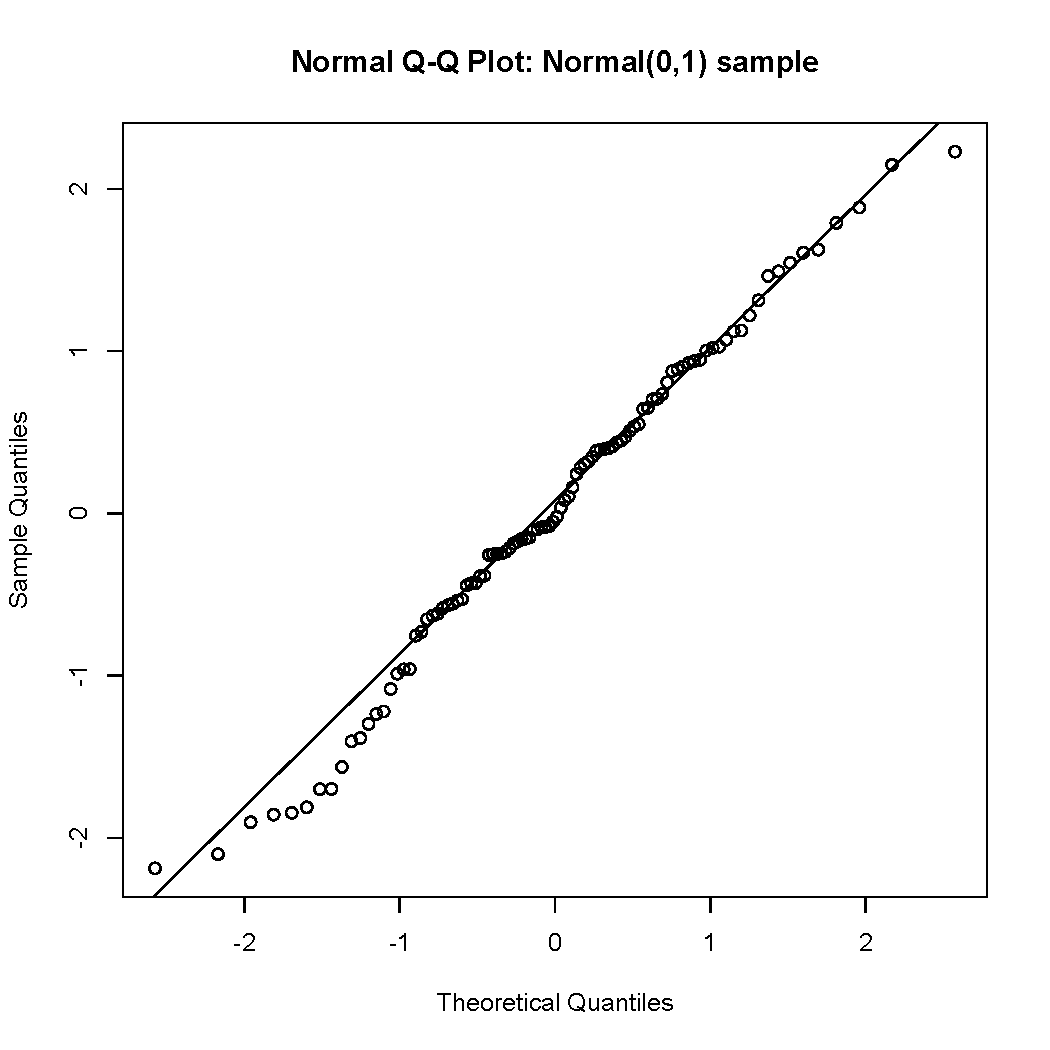
\includegraphics{nqqplot-normal}}
%\end{minipage}
%\hfill
%\begin{minipage}{0.45\linewidth}
%\resizebox{\linewidth}{!}{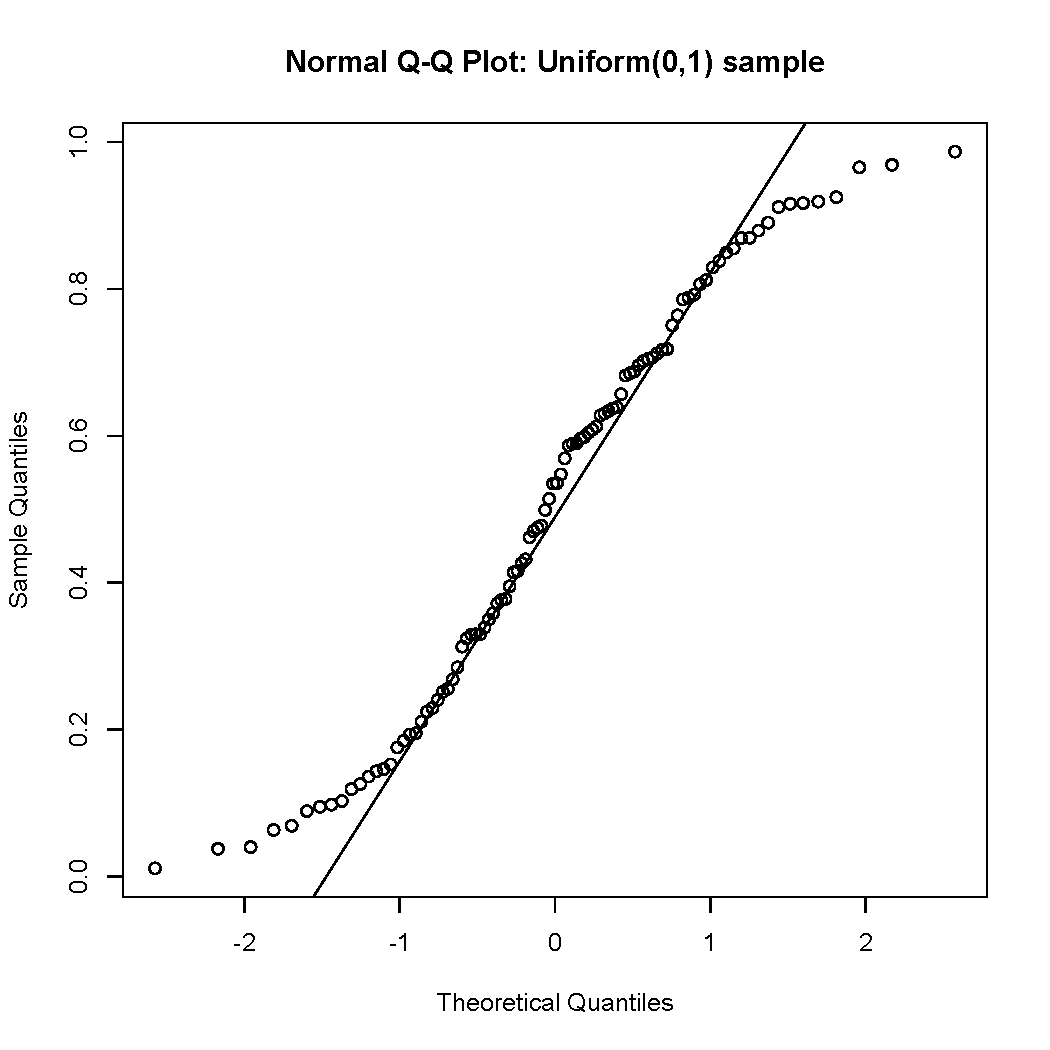
\includegraphics{nqqplot-uniform}}
%\end{minipage}
%\end{minipage}
\begin{figure}[ht]
\centering
\begin{tabular}{cc}
	\begin{subfigure}{0.45\textwidth}
	\resizebox{\linewidth}{!}{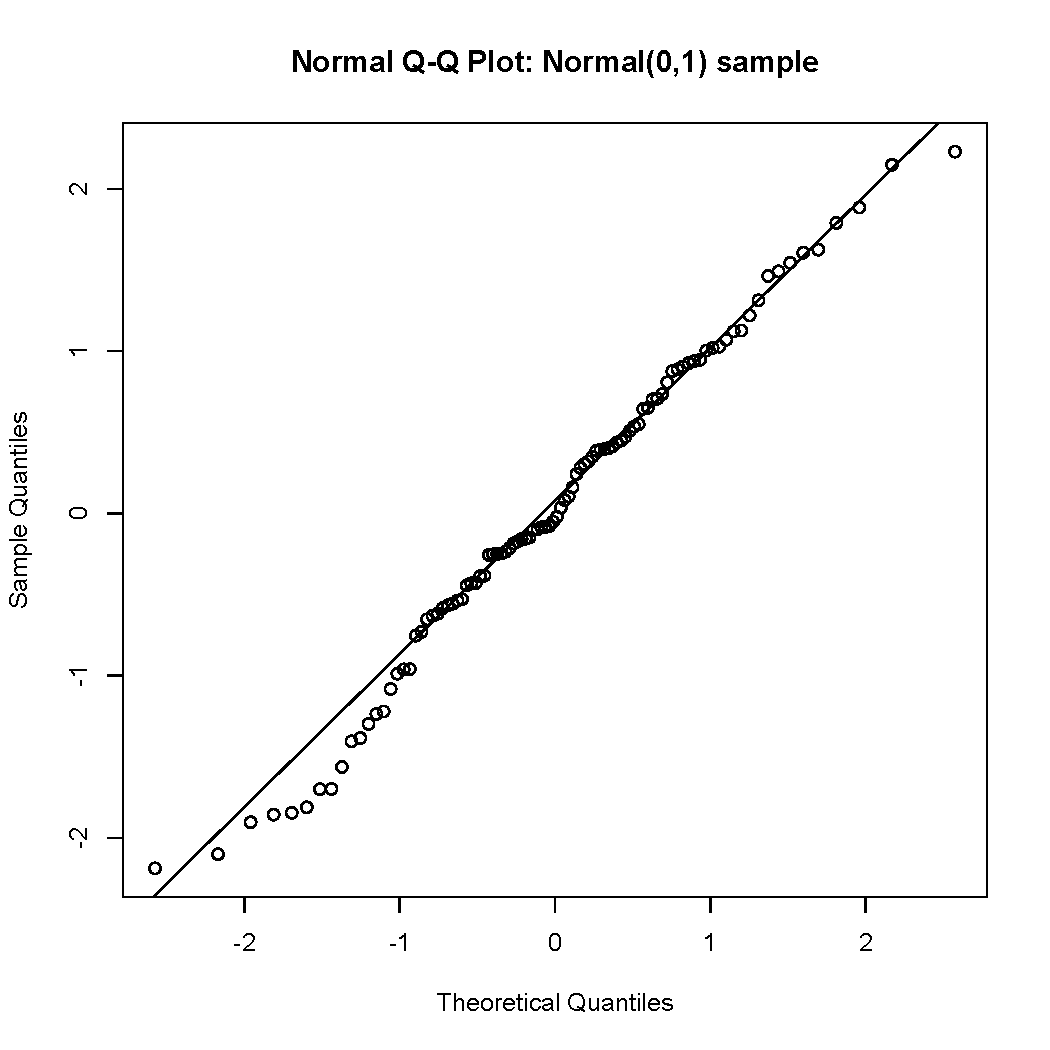
\includegraphics{nqqplot-normal}}
	\end{subfigure}
&
	\begin{subfigure}{0.45\textwidth}
	\resizebox{\linewidth}{!}{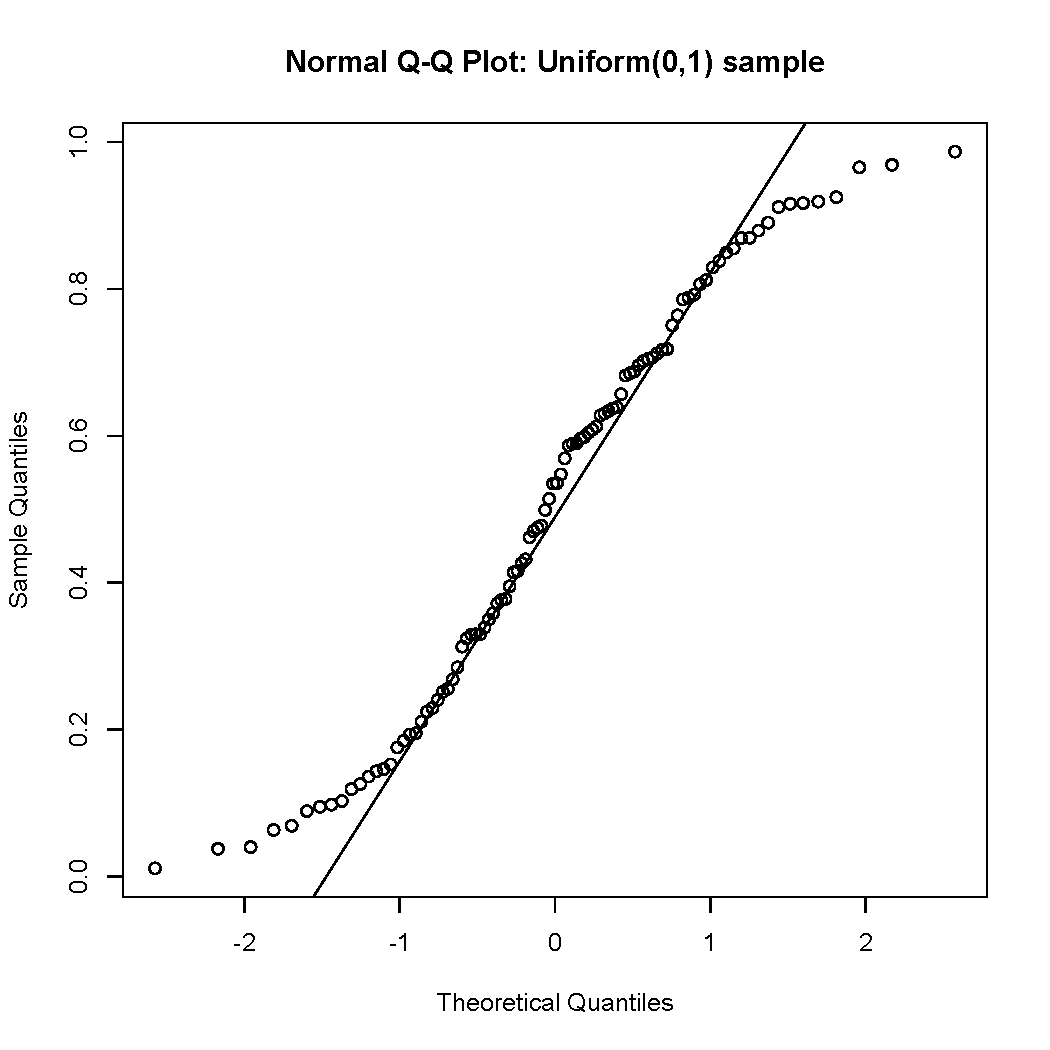
\includegraphics{nqqplot-uniform}}
	\end{subfigure}
\end{tabular}
\caption{Q-Q plots for testing normality.\label{fig:qq}}
\end{figure}

\end{example} 

% exercise (symmetric distributions)
\begin{exercise}
\begin{questions}
\question
Let $X$ be a random variable, let $F_X$ be its CDF and suppose that its distribution is symmetric about $a$.  Using the fact that $X-a$ and $-(X-a)$ have the same distribution, show that any location functional satisfies $T(F_X)=a$. 
\begin{answer}
Because $T$ is a location functional,
\[
T(F_{X-a}) = T(F_X)-a \qquad\text{and}\qquad T(F_{-(X-a)}) = -T(F_X)+a.
\]
Because $X-a$ and $-(X-a)$ have the same distribution, these are equal so $T(F_X)=a$, as required.
\end{answer}

\question %median and IQR
\begin{parts}
\part % median
Show that the median is a location functional.
\begin{answer}
Let $Y=a+bX$. Then
\[
F_{a+bX}(y) = \begin{cases}
	F_X\left(\frac{y-a}{b}\right)		& \text{ if $b>0$,} \\
	1 - F_X\left(\frac{y-a}{b}\right)	& \text{ if $b<0$.} 
\end{cases}
\]
Let $T(F_X)=F_X^{-1}(1/2)$ be the median functional. Then $F_X\big[T(F_X)\big] = 1/2$ so for $b>0$, 
\[
F_{a+bX}\big[a+bT(F_X)\big] = F_X\left[\frac{a+bT(F_X) - a}{b}\right] = F_X\big[T(F_X)\big] = 1/2,
\]
and for $b<0$, 
\[
F_{a+bX}\big[a+bT(F_X)\big] = 1 - F_X\left[\frac{a+bT(F_X) - a}{b}\right] = 1 - F_X\big[T(F_X)\big] = 1 - 1/2 = 1/2.
\]
In either case we have 
\[
T(F_{a+bX}) = F_{a+bX}^{-1}(1/2) = a+bT(F_X),
\]
so the median is a location functional, as required.
\end{answer}

\part % IQR
Show that the inter-quartile range is a scale functional.
\begin{answer}
Let $L(F_X) = F_X^{-1}(1/4)$ and $U(F_X)=F_X^{-1}(3/4)$ be the lower-quartile and upper-quartile functionals respectively. Then
\[
F_X\big[L(F_X)\big] = 1/4 \quad\text{and}\quad F_X\big[U(F_X)\big] = 3/4.
\]
For $b>0$, 
\begin{align*}
F_{a+bX}\big[a+bL(F_X)\big]
	& = F_X\left[\frac{a+bL(F_X) - a}{b}\right] = F_X\big[L(F_X)\big] = 1/4,\\
F_{a+bX}\big[a+bU(F_X)\big]
	& = F_X\left[\frac{a+bU(F_X) - a}{b}\right] = F_X\big[U(F_X)\big] = 3/4,\\
\end{align*}
Thus $L(F_{a+bX}) = F_{a+bX}^{-1}(1/4) = a+bL(F_X)$ and $U(F_{a+bX}) = F_{a+bX}^{-1}(3/4) = a+bU(F_X)$.

\bigskip
The inter-quartile range functional is $T(F_X)=U(F_X)-L(F_X)$, so
\[
T(F_{a+bX}) 
	= F_{a+bX}^{-1}(3/4) - F_{a+bX}^{-1}(1/4) 
	= \big[a+bU(F_X)\big] - \big[a + bL(F_X)\big]
	= b\big[U(F_X)-L(F_X)\big]
	= bT(F_X).
\]
Thus the inter-quartile range is a scale functional, as required.
\end{answer}
\end{parts}
\end{questions}
\end{exercise}



% !TEX root = main.tex

%-------------------------------------------------
\section{One-sample tests}\label{sec:np_one_sample_tests}

%-------------------------------------------------
\subsection{The sign test}\label{sec:signtest}

Let $X$ be a continuous random variable with an unknown median $\eta$. The sign test is a non-parametric method for testing hypotheses about $\eta$.

%%-----------------------------
%\subsection{The median}
%The non-parametric methods we consider are based on the \emph{median} of an unknown distribution.
%
%\begin{definition}
%A \emph{median} of a random variable $X$ is a real number $\eta$ satisfying
%\[
%\prob(X\leq\eta)\,\geq\frac{1}{2} \quad\text{and}\quad \prob(X\geq\eta)\,\geq\frac{1}{2}.
%\]
%If $X$ is a continuous random variable, its median is uniquely defined,
%\[
%\prob(X\leq\eta) = \prob(X\geq\eta) = \frac{1}{2}.
%\]
%\end{definition}
%
%\begin{example}
%Consider the random sample $\{1, 2, 2, 2, 3, 14\}$.
%\bit
%\it The sample median is $\hat{\eta} = 2$; the sample mean is $\hat{\mu}  = 4$.
%\eit
%In this case, $\hat{\eta}$ provides a better indicator of centrality than $\hat{\mu}$.
%\end{example}

%-----------------------------
\subsubsection{The test statistic}

Let $X_1,X_2,\ldots,X_n$ be a random sample from the distribution of $X$ and consider the null hypothesis $H_0:\eta=\eta_0$ against a suitable alternative. If $H_0$ is correct then approximately half of the observations should be smaller than $\eta_0$ and approximately half should be larger than $\eta_0$.

\begin{definition}
The sign test statistic $S^{+}_n$ is the number of observations larger than $\eta_0$: 
\[
S^{+}_n = \sum_{i=1}^n Z_i \quad\text{where}\quad Z_i=I(X_i>\eta_0).
\]
\end{definition}

We also define the complementary statistic $S^{-}_n = \displaystyle\sum_{i=1}^n (1-Z_i)$ which is the number of observations smaller than $\eta_0$. Note that $S^{+}_n + S^{-}_n = n$.

\bigskip
Because the observations are independent, the distribution of our test statistic under $H_0$ is
\[
S^{+}_n\sim\text{Binomial}(n,0.5).
\]
\bit
\it Small values of $S^{+}_n$ support the alternative $H_1:\eta < \eta_0$.
\it Large values of $S^{+}_n$ support the alternative $H_1:\eta > \eta_0$.
\eit

% example: sign test (one sample)
\begin{example}
The following are measurements of the breaking strength of a certain kind of two-inch cotton ribbon.
\[\begin{array}{cccccccccc}
163 & 165 & 158 & 189 & 161 & 171 & 158 & 151 & 169 & 162 \\
163 & 139 & 172 & 165 & 148 & 166 & 172 & 163 & 187 & 173 \\
\end{array}\]
Conduct a sign test to decide between $H_0:\eta=160$ and $H_1:\eta>160$ at significance level $\alpha=0.05$. 
\end{example}

\begin{solution}
First we must assume that the distribution of the breaking strength is continuous.
\small
\[\begin{array}{cccccccccc} \hline
163 & 165 & 160 & 189 & 161 & 171 & 158 & 151 & 169 & 162 \\
+ & + & - & + & + & + & - & - & + & + \\ \hline
163 & 139 & 172 & 165 & 148 & 166 & 172 & 163 & 187 & 173 \\
+ & - & + & + & - & + & + & + & + & + \\ \hline
\end{array}\]
\normalsize
\bit
\it We have $n=20$ signs: under the null hypothesis, $S^{+}_n\sim\text{Binomial}(20,0.5)$.
\it The observed value of the test statistic $s^{+}_n=15$. 
\it From tables we find that $\prob_{H_0}(S^{+}_n\geq 15) = 1 - 0.9793 = 0.0207$ approx. 
\it Thus we reject $H_0$ at significance level $\alpha=0.05$.
\eit
\end{solution}

% example: sign test (paired samples)
\begin{example}[Sign test for paired samples]
To evaluate a new traffic-control system, the number of accidents that occurred at 12 dangerous junctions were recorded during the four weeks prior to the installation of the new system, and for the four weeks after its installation. The following data were obtained.
\small
\[\begin{array}{|l|rrrrrrrrrrrr|} \hline
\text{Junction}	& \phantom{1}1 & \phantom{1}2 & \phantom{1}3 & \phantom{1}4 & \phantom{1}5 & \phantom{1}6 & \phantom{1}7 & \phantom{1}8 & \phantom{1}9 & 10 & 11 & 12 \\ \hline
\text{Before}	& 3 & 5 & 2 & 3 & 3 & 3 & 0 & 4 & 1 &  6 &  4 &  1 \\
\text{After}	& 1 & 2 & 2 & 2 & 2 & 0 & 2 & 3 & 3 &  4 &  1 &  0 \\ \hline
\end{array}\]
\normalsize
Use a sign test to evaluate the claim that the new system is more effective than the old system.
\end{example}

\begin{solution}
Let $\eta_1$ and $\eta_2$ denote the median number of accidents before and after the new system was installed, respectively. We test $H_0:\eta_1=\eta_2$ against $H_1:\eta_1 > \eta_2$.
\[\begin{array}{|l|rrrrrrrrrrrr|} \hline
\text{Junction}	& \phantom{1}1 & \phantom{1}2 & \phantom{1}3 & \phantom{1}4 & \phantom{1}5 & \phantom{1}6 & \phantom{1}7 & \phantom{1}8 & \phantom{1}9 & 10 & 11 & 12 \\ \hline
%\text{Before}		& 3 & 5 & 2 & 3 & 3 & 3 & 0 & 4 & 1 &  6 &  4 &  1 \\
%\text{After}		& 1 & 2 & 2 & 2 & 2 & 0 & 2 & 3 & 3 &  4 &  1 &  0 \\ \hline
\text{Difference}	& + & + & 0 & + & + & + & - & + & - &  + &  + &  + \\ \hline
\end{array}\]

\bit
\it We have $n=11$ observations (one discarded) so $S^{+}_n\sim\text{Binomial}(11,\theta)$ under $H_0$.
\it The value of the test statistic is $s^{+}_n = 9$.
\it Under $H_0:\theta=0.5$, from tables we obtain $\prob_{0.5}(S^{+}_n\geq 9) = 1 - 0.9673 = 0.0327$.
\it At $\alpha=0.05$ we reject $H_0$ and conclude that the system has indeed reduced the number of accidents.
\it At $\alpha=0.01$ we retain $H_0$ and conclude that there is insufficient evidence to support the claim.
\eit
\end{solution}

%-----------------------------
\subsubsection{Normal approximation}

By the central limit theorem, if $X\sim\text{Binomial}(n,\theta)$ then for large $n$,
\[
X\sim N\big(n\theta,n\theta(1-\theta)\big) \text{\quad approx.}
\]
If $H_0:\theta=0.5$ is correct, the distribution of the test statistic is $S^{+}_n\sim N(n/2,n/4)$ approx.

% continuity correction
\begin{definition}[The continuity correction]
Let $X$ be a discrete random variable, taking values in the set $\{0,\pm 1,\pm 2,\ldots\}$. If the distribution of a continuous random variable $Y$ is taken as an approximation of the distribution of $X$, we set
\[
\prob(X=k) = \prob\left(k - \frac{1}{2} < Y < k + \frac{1}{2}\right).
\] 
\end{definition}
This means that 
\bit
\it $\prob(X < k) = \prob(Y\leq k-1/2)$ and $\prob(X\leq k) = \prob(Y\leq k+1/2)$,
\it $\prob(X\geq k) = \prob(Y\geq k-1/2)$ and $\prob(X > k) = \prob(Y\geq k+1/2)$
\eit

% example: sign test (large sample)
\begin{example}[Sign test for large samples]
The following data are the amounts of sulphur oxide (in tonnes) emitted by a large industrial plant over a period of 40 days.
\[\begin{array}{cccccccccc}
17 & 15 & 20 & 29 & 19 & 18 & 22 & 25 & 27 &  9 \\
24 & 20 & 17 &  6 & 24 & 14 & 15 & 23 & 24 & 26 \\
19 & 23 & 28 & 19 & 16 & 22 & 24 & 17 & 20 & 13 \\
19 & 10 & 23 & 18 & 31 & 13 & 20 & 17 & 24 & 14
\end{array}\]
Construct a sign test of size $\alpha=0.01$ to evaluate $H_0:\eta=21.5$ against $H_1:\eta<21.5$.
\end{example}

\begin{solution}
Assume that sulphur oxide emissions per day has a continuous distribution. The sign test statistic is
\[
S^{+}_n = \sum_{i=1}^n I(X_i>21.5).
\]
and because the sample is relatively large, $S^{+}_n\sim N(n/2,n/4)$ approx.

\bigskip
Using the continuity correction (for a lower-tailed test), we have the test statistic
\[
Z = \displaystyle\frac{(S^{+}_n+1/2)-n/2}{\sqrt{n/4}} \sim N(0,1) \text{ approx.}
\]
Here, we have $n=40$ and $s^{+}_n=16$ (the number values exceeding $\mu_0 = 21.5$), so the value of the test statistic is
\[
z = \frac{16.5 - 20}{\sqrt{10}} = -1.1068.
\]
From tables, the (lower-tail) critical value of $N(0,1)$ at $\alpha=0.01$ is $z_c = \Phi^{-1}(0.01) = -2.33$ approx. Thus we retain $H_0$ and conclude that the median amount of sulphur oxide emitted by the plant is not less than $21.5$ tons per day.
\end{solution}

\begin{exercise}
\begin{questions}

\question % flies
The biting rate of a particular species of fly was investigated. The biting rate is defined as the number of flies biting a volunteer during $15$ minutes of exposure. The species is known to have a median biting rate of $5$ bites per $15$ minutes. It is hypothesized that the median biting range is higher in bright, sunny weather. To test the hypothesis, a total of $122$ volunteers were exposed to flies on a sunny day, of which $95$ experienced biting rates greater than $5$.
State the null and alternative hypotheses for the test, and state your conclusion for $\alpha = 0.01$.
\begin{answer}
Let $\eta$ deonte the (true) median biting rate. 
\par
The hypothesis test is $H_0:\eta=5$ against, $H_1:\eta>5$.
\par
The test statistic is $S_n^{+} = 95$ where $n=122$. 

\bigskip
Under the null hypothesis, $\prob(S_{122}^{+}\geq 95) = \prob\big[\text{Binomial}(122,0.5) \geq 95\big]$.

\bigskip
Since $n$ is large, we use the normal approximation: under the null hypothesis,
\[
Z = \frac{(S_n^{+}-1/2) - n/2}{\sqrt{n/4}} \sim N (0,1) \quad\text{approx.}
\]
In this case, the test statistic is
\[
z = \frac{94.5 - 61}{\sqrt{30.5}} = 6.0659.
\]
An approximate $p$-value is $\prob(Z>6.6059) < 0.001$, so we reject $H_0$ at $\alpha=0.01$.
\end{answer}

\question % sign-test v z-test
Let $X\sim N (\mu,1)$ where $\mu$ is unknown and suppose we wish to test the simple null hypothesis $H_0:\mu=0$ against the simple alternative $H_1:\mu=0.5$. A random sample of 9 observations is taken from the distribution of $X$ and the number $S^{+}$ of positive values is counted.
\ben
\it % << (i)
A sign test rejects the null hypothesis if $S^{+}$ exceeds $6$. Find the size and power of the test.
\it % << (ii)
Construct a test based on the sample mean of the observations which has the same significance level as the sign test described above. Find the power of the test, and explain why this is higher than the power of the sign test.
\een

\begin{answer}
\ben
\it % << (i)
Under the null hypothesis, $S^{+}\sim\text{Binomial}(9, 0.5)$. The size of the test is
\[
\alpha = \prob_{\mu_0}(S^{+}>6) = \prob\big(\text{Binomial}(9,0.5)>6\big) \approx 0.0898 \text{ (from tables)}.
\]
Under $H_1:\mu=0.5$ we have $X\sim N(0.5,1)$, so the probability that an observataion takes a positive value under $H_1$ is
\[
\prob_{\mu_1}(X > 0) 
	= \prob\big(X > 0 \text{ where } X\sim N(0.5,1)\big) 
	= \prob\big(Z > -0.5 \text{ where } Z\sim N(0,1)\big) 
	\approx 0.69146 \quad\text{(from tables).}
\]
The power of the test to detect the alternative $H_1:\mu=0.5$ is therefore
\[
\gamma(0.5) = \prob_{\mu_1}(S^{+}>6) = \prob\big[\text{Binomial}(9,0.6915) > 6\big] = \prob\big[\text{Binomial}(9,0.0.3085) < 3\big] 
\]
where the second equality follows by the fact that 
\[
\prob\big[\text{Binomial}(n,p) > k\big] = \prob\big[\text{Binomial}(n,1-p) < n-k\big].
\]
From tables, we find that 
\[
\prob[\text{Binomial}(9,0.30)\leq 2\big] \approx 0.4628  \quad\text{and}\quad \prob[\text{Binomial}(9,0.35)\leq 2\big] \approx 0.3373.
\]
To find the required probability, we interpolate between these values:
\begin{align*}
\prob\big[\text{Binomial}(9,0.3085)\leq 2\big]
	& \approx \prob\big[\text{Binomial}(9,0.30)\leq 2\big] \\
	& \qquad + \left(\frac{0.3085 - 0.30}{0.35 - 0.30}\right)\left(\prob\big[\text{Bino}(9,0.35)\leq 2\big]-\prob\big[\text{Bino}(9,0.30)\leq 2\big]\right) \\
	& = 0.4628 - (0.1708\times 0.1255) \\
	& = 0.4414.
\end{align*}	
Alternatively, we can use the normal approximation: if $Y\sim \text{Binomial}(9,0.6915)$ then $\expe(Y) = 6.2231$ and $\var(Y) = 1.9201$. Using the continuity correction,
\[
\prob\big[\text{Binomial}(9,0.6915) > 6\big]
	\approx \prob\left[ N (0,1) > \frac{6.5-6.2231}{\sqrt{1.9201}}\right]
	= \prob\big(N(0,1)> 0.1998\big) 
%	= 1 - 0.5793 
	\approx 0.4207.
\]	
\item % (ii)
Let $\bar{X}$ denote the sample mean, and consider the $z$-test, where $H_0:\mu=0$ is rejected in favour of $H_1:\mu=0.5$ if $\bar{X} > c$, with $c$ chosen to give the required significance level. Here we require $\alpha = 0.0898$, so we need
\[
\prob_{\mu_0}(\bar{X} > c) = 0.0898.
\]
Under $H_0$ we have $X_i\sim N (0,1)$, so $\expe(\bar{X})=0$ and $\var(\bar{X})=1/9$. Thus $\bar{X}\sim N (0,1/9)$, so the critical value $c$ satisfies
\[
\prob\left( N (0,1) > \frac{c}{\sqrt{1/9}}\right) = 0.0898,
\]
i.e.\ $1-\Phi(3c) = 0.0898$, or $\Phi(3c) = 0.9102$. From tables, $\Phi(1.34076) = 0.91$ and $\Phi(1.40507)= 0.92$. Interpolating linearly between these values gives
\[
3c = 1.34076 + 0.02(1.40507 - 1.34076) = 1.342,
\]
so $c\approx 0.447$. The statistical power is 
\begin{align*}
\gamma(0.5) = \prob_{H_1}(\bar{X} > 0.447) 
	& = \prob\big(N(0.5,1/9) > 0.447\big) \\
	& = \prob\big(N(0,1) > 3(0.447 - 0.5)\big) \\
	& = \prob\big(N(0,1) > -0.159)\big) \\
	& \approx 0.564 \quad\text{(from tables).}
\end{align*}
This is higher than the power of the sign test (which is approximately $0.43$), because the $z$-test takes account of the magnitude of the observations, as well as their signs. If the data really do come from a normal distribution, the $z$-test is more powerful than the sign test for detecting $H_1:\mu=0.5$ against $H_0:\mu=0$.
\een
\end{answer}
\end{questions}
\end{exercise}


%-------------------------------------------------
\subsection{The Wilcoxon signed-rank test}\label{sec:wsr_test}

The Wilcoxon signed rank test is an extension of the sign test.
\bit
\it The sign test counts the \emph{number} of observations which are larger than some fixed value.
\it The WSR test also considers the \emph{relative size} of these observations.
\eit

%-----------------------------
%\subsubsection{Ranks}

\begin{definition}
For a random sample $X_1,\ldots,X_n$, the \emph{rank} of observation $X_i$ is its position in the sequence of observations sorted in ascending order:
\[
R(X_i) = \sum_{j=1}^n I(X_j \leq X_i)
\]
\end{definition}

Note that the sum of the ranks is always equal to the sum of the first $n$ positive integers:
\[
\displaystyle \sum_{i=1}^n R(X_i) = \sum_{i=1}^n i = \frac{1}{2}n(n+1).
\]

\begin{remark}[Ties]
If two or more observations have the same value, they are said to be \emph{tied}. If the distribution is continuous, ties occur with probability zero. Ties often occur in practical applications however, due to the limited precision of measurements. To deal with ties, the usual approach is to assign an \emph{average rank} to each of the tied observations. For example, if there are $m-1$ observations strictly smaller than $X_i=X_j$, we set
\[
R(X_i) = R(X_j) = \frac{m+(m+1)}{2} = m+\frac{1}{2}.
\]
\end{remark}

%-----------------------------
\subsubsection{The test statistic}

Let $X$ be a continuous random variable whose distribution is \emph{symmetric} and whose median $\eta$ is unknown, and let $X_1,X_2,\ldots,X_n$ be a random sample from the distribution of $X$. 
Without loss of generality, we consider the null hypothesis $H_0:\eta=0$:
\bit
\it for a single sample $X_1,X_2,\ldots,X_n$, the null hypothesis $H_0:\eta=\eta_0$ reduces to $H_0:\eta=0$ by looking at the differences $D_i = X_i - \eta_0$;
\it For paired samples $X_1,X_2,\ldots,X_n$ and $Y_1,Y_2,\ldots,Y_n$, the null hypothesis $H_0:\eta_1=\eta_2$ reduces to $H_0:\eta=0$ by looking at the differences $D_i = X_i - Y_i$.
\eit

% definition: wsr statistic
\begin{definition}
For the null hypothesis $H_0:\eta=0$, the \emph{Wilcoxon signed rank} (WSR) statistic is 
\[
W^{+}_n = \sum_{i=1}^n R_i Z_i \quad\text{where}\quad R_i = \sum_{j=1}^n I(|X_j|\leq |X_i|) \quad\text{and}\quad Z_i=I(X_i>0).
\]
\end{definition}
\bit
\it $R_i$ is the rank of $|X_i|$ in the sample of absolute values $|X_1|,|X_2|,\ldots,|X_n|$;
\it $Z_i=1$ if $X_i>0$, otherwise $Z_i=0$.
\eit

We also define the complementary statistic $W^{-}_n = \displaystyle\sum_{i=1}^n R_i(1-Z_i)$. Note that
\[
W^{+}_n + W^{-}_n = \sum_{i=1}^n R_i = \sum_{i=1}^n i = \frac{1}{2}n(n+1).
\]

%% test procedure
%The WSR test procedure is as follows:
%\ben
%\it Compute the differences $D_i = X_i - \eta_0$ (single sample) or $D_i=X_i-X'_i$ (matched pairs).
%\it Compute absolute differences $|D_i|$ and record the sign of $D_i$.
%\it Compute the ranks $R_i$ of the absolute differences $|D_i|$.
%\it Compute the the sum of the ranks of those $|D_i|$ having positive sign. 
%\een
%The final step yields the test statistic $W^{+}_n$.

% example
\begin{example}
A study of the effects of smoking by mothers on the birthweight of their children involved 12 pairs of mothers. The pairs of mothers were selected so that they were as similar as possible, except that one mother of each pair was a smoker and the other was not. The birthweights (in kilograms) of the babies were as follows.
\small
\[\begin{array}{l|cccccccccccc} \hline
\text{Pair}			& 1      &  2     & 3      & 4      & 5      & 6      & 7      & 8      & 9      & 10     & 11     & 12 		\\ \hline
\text{Non-smoker}	& 3.22   & 4.48   & 3.90   & 3.47   & 3.07   & 3.23   & 4.25   & 3.31   & 3.33   & 3.78   & 3.18   & 4.60  	\\ 
\text{Smoker}		& 3.00   & 4.27   & 3.95   & 3.32   & 2.51   & 2.77   & 4.02   & 3.41   & 3.39   & 3.88   & 3.18   & 4.37 	\\ \hline
\end{array}\]
\normalsize
Do these data support the claim that mothers who smoke tend to have babies with smaller birthweights than those who do not? 
\end{example}

\begin{solution}
The data are in matched pairs so we compute the differences $D_i=X_i-Y_i$, where $X_1,X_2,\ldots,X_n$ are the birthweights for non-smokers and $Y_1,Y_2,\ldots,Y_n$ are the corresponding birthweights for smokers. The test then becomes
\[
H_0:\eta = 0 \quad\text{against}\quad H_1:\eta > 0,
\]
where $\eta$ is the (true) median difference between birthweights for the non-smoking group and birthweights for the smoking group.

\small
\[\begin{array}{|c|cccccccccccc|} \hline
i			& 1      &  2     & 3      & 4      & 5      & 6      & 7      & 8      & 9      & 10     & 11     & 12   	\\ \hline
X_i			& 3.22   & 4.48   & 3.90   & 3.47   & 3.07   & 3.23   & 4.25   & 3.31   & 3.33   & 3.78   & 3.18   & 4.60 	\\ 
X'_i		& 3.00   & 4.27   & 3.95   & 3.32   & 2.51   & 2.77   & 4.02   & 3.41   & 3.39   & 3.88   & 3.18   & 4.37	\\ \hline
D_i			& 0.22   & 0.21   & -0.05  & 0.15   & 0.56   & 0.46   & 0.23   & -0.10  & -0.06  & -0.10  & 0.00  	& 0.23	\\
|D_i|		& 0.22   & 0.21   &  0.05  & 0.15   & 0.56   & 0.46   & 0.23   &  0.10  &  0.06  &  0.10  & 0.00  	& 0.23	\\ \hline
\text{sgn}(D_i)	& +      & +      & -      & +      & +      & +      & +      & -      & -      & -      &      	& +  	\\ 
%R(|D_i|)		& 8      & 7      & 2      & 6      & 12     & 11     & 9.5    &  4.5   &  3     &  4.5   & 0     	& 9.5  	\\ \hline
R(|D_i|)		& 7      & 6      & 1      & 5      & 11     & 10     & 8.5    &  3.5   &  2     &  3.5   &      	& 8.5  	\\ \hline
\end{array}\]
\vspace*{-2ex}\normalsize
\bit
\it The zero difference is discarded, leaving $n=11$ non-zero differences.
\it Ties are replaced by the average of the corresponding ranks.
\eit
From the data, $W^{+}_n = 56$ and $W^{-}_n = 10$. \Big[Check: $W^{+}_n + W^{-}_n = 66 = \frac{1}{2}n(n+1)$.\Big]
\bit
\it Large values of $W^{+}_n$ support the alternative hypothesis, $H_1:\eta > 0$. 
\it From tables, the upper-tail critical value of $W^{+}_n$ for $n=11$ at $\alpha=0.05$ is $w_c = 52$. 
\eit
Since $W^{+}_n > w_c$, we reject the null hypothesis and conclude that mothers who smoke tend to have babies with smaller birthweights than those who do not. 
\end{solution}


%-----------------------------
\subsubsection{Mean and variance of $W^{+}_n$}

% theorem: mean and variance of W+
\begin{theorem}
Let $X_1,X_2,\ldots,X_n$ be a random sample from a continuous distribution whose density function is symmetric about its mean. Under the null hypothesis $H_0:\eta=0$, 
\[
\expe(W^{+}_n) = \frac{n(n+1)}{4} \qquad\text{and}\qquad \var(W^{+}_n)	= \frac{n(n+1)(2n+1)}{24}.
\]
\end{theorem}

\begin{proof}
Recall that 
\[
W^{+}_n = \sum_{i=1}^n R_i Z_i \quad\text{where}\quad R_i = \sum_{j=1}^n I(|X_j|\leq |X_i|) \quad\text{and}\quad Z_i=I(X_i>0).
\]
%
%$W^{+}_n = \sum_{i=1}^n R_iZ_i$, where $R_i=R(|X_i|)$ and $Z_i = I(X_i > 0)$.
Under $H_0:\eta=0$ we have $Z_i\sim\text{Bernoulli}(1/2)$ and hence $\expe(Z_i)=1/2$ and $\var(Z_i)=1/4$. 

\begin{align*}
\expe(W^{+}_n) 
	& = \sum_{i=1}^n R_i\expe(Z_i) 
	= \frac{1}{2}\sum_{i=1}^n R_i
	= \frac{1}{2}\sum_{i=1}^n i
	= \frac{1}{4}n(n+1). \\
\var(W^{+}_n)
	& = \sum_{i=1}^n R_i^2 \var(Z_i) 
	= \frac{1}{4}\sum_{i=1}^n R_i^2
	= \frac{1}{4}\sum_{i=1}^n i^2
	= \frac{1}{24}n(n+1)(2n+1).
\end{align*}
\end{proof}

%\begin{remark}
%\bit
%\it
%In practice, the sum of the squares of the ranks is equal to the sum of the squares of the first $n$ natural numbers only if there are no ties and no zeros (i.e.\ observations that are exactly equal to $\eta_0$).
%\it A correction for ties is
%\[
%\var(W^{+}_n) = \frac{1}{24}n(n+1)(2n+1) - \frac{1}{48}\sum t(t^2-1)
%\]
%where $t$ is the number of tied observations (e.g.\ $t=2$ if there are two identical observations) and the summation is over the number of sets of tied observations.
%\eit
%\end{remark}

%-----------------------------
\subsubsection{Normal approximation}
$W^{+}_n$ is the sum of random variables and (although the random variables are not independent) it satisfies the central limit theorem. Under $H_0:\eta=0$, and provided $n$ is sufficiently large, the distribution of $W^{+}_n$ is 
\[
W^{+}_n \sim N\left(\frac{1}{4}n(n+1), \frac{1}{24}n(n+1)(2n+1)\right) \text{\quad approx.}
\]

The continuity correction should be applied when defining the test statistic.
\bit
\it Lower-talied test:
\[
Z = \frac{(W^{+}_n +\frac{1}{2})- \frac{1}{4}n(n+1)}{\sqrt{\frac{1}{24}n(n+1)(2n+1)}}\sim N(0,1) \quad\text{approx.}
\]
\it Upper-talied test:
\[
Z = \frac{(W^{+}_n -\frac{1}{2})- \frac{1}{4}n(n+1)}{\sqrt{\frac{1}{24}n(n+1)(2n+1)}}\sim N(0,1) \quad\text{approx.}
\]
\eit

%-----------------------------
\subsubsection{Exact distribution of $W^{+}_n$ under $H_0$}

The exact distribution of $W^{+}_n$ under $H_0$ can be obtained for small $n$ by a recurrence relation. The base case is $n=1$ (a single observation), for which $W^{+}_1\in\{0,1\}$ and under $H_0:\eta=0$,
\[
\prob(W^{+}_1 = 0) = \frac{1}{2} \quad\text{and}\quad \prob(W^{+}_1 = 1) = \frac{1}{2}.
\]
%
%
%\bit
%\it For $n = 2$, the set of ranks is $\{1,2\}$ so $W^{+}_2$ takes values in the set $\{0,1,2,3\}$. Under $H_0:\eta=0$, 
%%\small
%\[\begin{array}{|c|cccc|}\hline
%\text{Ranks}			& \{-1,-2\}	& \{+1,-2\}	& \{-1,+2\}	& \{+1,+2\}	\\ \hline
%k					& 0	& 1	& 2	& 3 \\ \hline
%\prob(W^{+}_2=k)		& 0.25		& 0.25		&  0.25		& 0.25 		\\ \hline
%\end{array}\]
%%\normalsize
%
%\it For $n=3$, the set of ranks is $\{1,2,3\}$, so $W^{+}_3$ takes values in the set $\{0,1,2,3,4,5,6\}$. Under $H_0:\eta=0$,
%%\small
%\[\begin{array}{|c|ccccccc|}\hline
%k				& 0		& 1		& 2		& 3 		& 4 		& 5 		& 6		\\ \hline
%\prob(W^{+}_3=k)	& 0.125	& 0.125	& 0.125	& 0.25	& 0.125	& 0.125	& 0.125	\\ \hline
%\end{array}\]
%%\normalsize
%\eit

% theorem
\begin{theorem}
Under $H_0:\eta=0$,
\[
\prob\big(W^{+}_{n+1}=k\big) = \frac{1}{2}\prob\big(W^{+}_n=k\big) + \frac{1}{2}\prob\big(W^{+}_n=k-(n+1)\big).
\]
%for $k=0,1,\ldots,\displaystyle\frac{1}{2}n(n+1)$ (and zero otherwise).
for $k=0,1,\ldots,\frac{1}{2}n(n+1)$, and zero otherwise.
\end{theorem}

\begin{proof}
\bit
\it Let $X_1,X_2,\ldots,X_n$ be a random sample from a continuous and symmetric distribution.
\it Let $R_i$ be the rank of $|X_i|$ among the absolute values $|X_1|,|X_2|,\ldots,|X_n|$:
\eit

Then $W^{+}_n$ can be written as
\[
W^{+}_n = \sum_{r=1}^n rU_r \qquad\text{where}\qquad U_{R_i} = \begin{cases} 1 & X_i > 0, \\ 0 & \text{otherwise.}\end{cases}
\]

\bit
\it $U_r$ indicates that the observation associated with rank $r$ has a positive sign.
\it Under the null hypothesis, $U_1,U_2,\ldots,U_n$ is a random sample from the $\text{Bernoulli}(1/2)$ distribution.
\eit

Let $G_n(t)$ denote the probability generating function of $W^{+}_n$:
\begin{align*}
G_n(t) 
	= \expe(t^{W^{+}_n})  
	= \expe(t^{\sum_{r=1}^n rU_r})
	& = \expe(t^{U_1}t^{2U_2}\cdots t^{nU_n}) \\
	& = \prod_{r=1}^n \expe(t^{rU_r}) \qquad\text{(by independence)} \\
	& = \prod_{r=1}^n \Big[t^0\,\prob(U_r=0) + t^r\,\prob(U_r=1)\Big] \\
	& = \prod_{r=1}^n \frac{1}{2}(1 + t^r). \\
\intertext{Hence,}
G_{n+1}(t) 
	& = \frac{1}{2}(1 + t^{n+1})G_n(t).
\end{align*}

By definition,
\begin{align*}
G_n(t)		= \sum_{k=0}^{\frac{1}{2}n(n+1)}\,\prob(W^{+}_n=k)t^k
\qquad\text{and}\qquad
G_{n+1}(t)	= \sum_{k=0}^{\frac{1}{2}(n+1)(n+2)}\,\prob(W^{+}_{n+1}=k)t^k.
\end{align*}

Thus,
\[
\sum_{k=0}^{\frac{1}{2}(n+1)(n+2)}\,\prob(W^{+}_{n+1}=k)t^k 
	= \frac{1}{2}(1+t^{n+1})\sum_{k=0}^{\frac{1}{2}n(n+1)}\,\prob(W^{+}_n=k)t^k,
\]

Comparing the coefficients of $t^k$ yields the required recurrence relation:
\[
\prob\big(W^{+}_{n+1}=k\big) = \frac{1}{2}\prob\big(W^{+}_n=k\big) + \frac{1}{2}\prob\big(W^{+}_n=k-(n+1)\big).
\]
This recurrence relation is used to compute the quantiles of $W^{+}_n$ listed in statistical tables.
\end{proof}


\begin{exercise}
\begin{questions}

\question
We wish to test the hypothesis that two treatments $A$ and $B$ are equivalent, against the alternative hypothesis that the responses to treatment $A$ tend to be larger than the responses to treatment $B$. We perform a paired difference experiment, and analyse the resulting data using the Wilcoxon signed rank test. The data is shown in the following table.
\[\begin{array}{|l|cccccccccc|}\hline
\text{Pair}	&  1 &  2 &  3 &  4 &  5 &  6 &  7 &  8 &  9 & 10 \\ \hline
$A$ 			& 54 & 60 & 98 & 43 & 82 & 77 & 74 & 29 & 63 & 80 \\
$B$ 			& 45 & 45 & 87 & 31 & 71 & 75 & 63 & 30 & 59 & 82 \\ \hline
\end{array}\]
State the null and alternative hypotheses for the test, and conduct the test at significance level $\alpha=0.05$.

\begin{answer}
\ben
\it % << (i)
Let $D_i=A_i-B_i$ denote the differences, and let $\eta$ denote the (true) median difference. We test the null hypothesis $H_0:\eta=0$ against the one-sided alternative $H_1:\eta>0$.
\it % << (ii)
The signed ranks are computed as follows:
\[\begin{array}{|l|cccccccccc|}\hline
\text{Pair}			&  1 &  2 &  3 &  4 &  5 &  6 &  7 &  8 &  9 & 10 \\ \hline
\text{Difference}	&  9 & 15 & 11 & 12 & 11 &  2 & 11 & -1 &  4 & -2 \\ \hline
\text{Signed Rank}	&  5 & 10 &  7 &  9 &  7 &2.5 &  7 & -1 &  4 & -2.5 \\ \hline
\end{array}\]
\bit
\it The Wilcoxon signed rank statistics are $W^{+} = 51.5$ and $W^{-}=3.5$. 
\it Check: $\frac{1}{2}n(n+1) = 55 = W^{+}+W^{-}$.
\it From tables, for a one-tailed test at $\alpha=0.05$ and $n=10$, the critical value is $w^{+}_c = 44$.
\it Thus we reject $H_0:\eta=0$ in favour of $H_1:\eta>0$, and conclude that responses to treatment $A$ tend to be larger than responses to treatment $B$.
\eit
\een
\end{answer}

\question
In a comparison of two populations $A$ and $B$, a paired difference experiment with $n=30$ pairs yields the Wilcoxon signed-rank statistic $w^{+}=354$.
\ben
\it Construct a test to determine whether or not population $A$ is located to the right of population $B$.
\it Conduct the test at $\alpha=0.05$.
\it Repeat part (2) using a normal approximation to the distribution of $W^{+}$.
\een

\begin{answer}
\ben
\it % << (i)
Let $\eta_A$ and $\eta_B$ denote the (true) medians of populations $A$ and $B$ respectively. To determine whether population $A$ is located to the right of population $B$, we test the null hypothesis $H_0:\eta_A=\eta_B$ against the alternative $H_1:\eta_A > \eta_B$. We could also define $\eta=\eta_A-\eta_B$ to be the difference between the two medians, in which case we would test $H_0:\eta=0$ agaianst $H_1:\eta>0$. 

\it % << (ii)
From tables, for a one-tailed test at $\alpha=0.05$ and $n=30$, the critical value is $w^{+}_c = 313$, so we reject $H_0$ in favour of $H_1$.

To compute an approximate $p$-value for the test, from tables (for $n=30$) we see that $w^{+}_c = 345$ at $\alpha=0.01$ and $w^{+}_c = 356$ at $\alpha=0.005$. Interpolating between these values, 
\[
\prob_{H_0}(W^{+}\geq 354) \approx 0.01 + \left(\frac{354-345}{356-345}\right)(0.005 - 0.01) = 0.0059.
\]

\it % << (ii)
The normal approximation is $\prob(W^{+}\geq w^{+}_c) \approx \prob(Z\geq z_c)$ where
\[
Z = \frac{(W^{+}-1/2) - \expe(W^{+})}{\sqrt{\var(W^{+})}} \sim N (0,1) \quad\text{approx.},
\]
Here, $\expe(W^{+})$ and $\var(W^{+})$ are respectively the mean and variance of $W^{+}$ under $H_0$. 
\par
In this case,
\[
\expe(W^{+}) = \frac{1}{4}n(n+1) = 232
\quad\text{and}\quad
\var(W^{+})  = \frac{1}{24}n(n+1)(2n+1) = 2363,
\]
so the test statistic is 
\[
z = \frac{353.5 - 232}{\sqrt{2363}} = 2.4994.
\]
\bit
\it At $\alpha=0.05$ we have $z_c = 1.645$, so we reject $H_0$. 
\it From tables, an approximate $p$-value for the test is $1-0.99379 = 0.0062$.
\eit
\een
\end{answer}

\question
To test whether or not a new diet actually results in weight loss, a researcher recruited nine subjects, measured their weight (in kilograms) before starting the diet, and then again after two months on the diet. The results are shown in the following table.
\[\begin{array}{|l|ccccccccc|} \hline
\text{Case}			&  1 &  2 &  3 &  4 &  5 &  6 &  7 &  8 &  9 \\ \hline
\text{Weight before }	& 55 & 50 & 54 & 43 & 62 & 61 & 56 & 48 & 53 \\
\text{Weight after }		& 47 & 40 & 52 & 43 & 51 & 62 & 50 & 47 & 56 \\ \hline
\end{array}\]

\begin{parts}
\part
Use a sign test with $\alpha=0.05$ to decide whether or not the diet results in weight loss.
\begin{answer}
Let $\eta$ denote the (true) median weight loss. 
\par
We evaluate $H_0:\eta = 0$ against the alternative $H_0:\eta > 0$.
\[\begin{array}{|l|ccccccccc|} \hline
\text{Case } (i)			&  1 &  2 &  3 &  4 &  5 &  6 &  7 &  8 &  9 \\ \hline
\text{Weight before }	& 55 & 50 & 54 & 43 & 62 & 61 & 56 & 48 & 53 \\
\text{Weight after }		& 47 & 40 & 52 & 43 & 51 & 62 & 50 & 47 & 56 \\ \hline
\text{Difference } (D_i)	&  8 & 10 &  2 &  0 & 11 & -1 &  6 &  1 & -3 \\ \hline
\text{Sign }				&  + &  + &  + &    &  + &  - &  + &  + &  - \\ \hline
%\text{Rank } (R_i)		&  6 &  7 &  3 &    &  8 &1.5 &  5 &1.5 &  4 \\ \hline
\end{array}\]
\bit
\it Exclude the zero difference, and take the sample size to be $n=8$.
\it $S_n^{+} = \sum_i I(D_i>0) = 6$.
\it $S_n^{-} = \sum_i I(D_i<0) = 2$. 
\it Check: $S_n^{+} + S_n^{-} = n$.
\eit
Under $H_0$, $S_n^{+}\sim\text{Binomial}(n,0.5)$. From tables,
\[
\prob_{H_0}(S_n^{+}\geq 6) = 1 - \prob_{H_0}(S_n^{+}\leq 5) = 1 - 0.8555 = 0.1445.
\]
At $\alpha=0.05$, we would decide to retain the null hypothesis $H_0:\eta=0$, and conclude that the diet results in no weight loss.
\end{answer}

\part
Repeat the analysis using the Wilcoxon signed rank test.
\begin{answer}
\[\begin{array}{|l|ccccccccc|} \hline
\text{Difference } (D_i)	&  8 & 10 &  2 &  0 & 11 & -1 &  6 &  1 & -3 \\ \hline
\text{Sign }				&  + &  + &  + &    &  + &  - &  + &  + &  - \\ \hline
\text{Rank } (R_i)		&  6 &  7 &  3 &    &  8 &1.5 &  5 &1.5 &  4 \\ \hline
\end{array}\]
\bit
\it $W^{+} = \sum_i R_i I(D_i>0) = 6 + 7 + 3 + 8 + 5 + 1.5 = 30.5$.
\it $W^{-} = \sum_i R_i I(D_i<0) = 1.5 + 4 = 5.5$.
\it Check: $W^{+} + W^{-} = \frac{1}{2}n(n+1)$.
\eit
From tables, critical values for an upper-tail test are
\bit
\it $w^{+}_c = 30$ at $\alpha=0.05$, and 
\it $w^{+}_c = 32$ at $\alpha=0.025$.
\eit
Thus at $\alpha=0.05$ we would reject the null hypothesis $H_0:\eta = 0$ in favour of the alternative $H_0:\eta > 0$, and conclude that the diet does indeed result in weight loss.
\end{answer}

\part
Briefly discuss the reasons why the tests lead to different conclusions.
\begin{answer}
The sign test takes no account of the fact that the average amount of weight lost by those whose weight decreased over the study period, is significantly greater than the average amount of weight gained by those whose weight increased over the study period. 
\end{answer}
\end{parts}

\end{questions}
\end{exercise}





